% !TeX spellcheck = en_GB

\documentclass[handout]{beamer}

\usepackage[utf8]{inputenc}
\usepackage[english]{babel}
\usepackage{tabularx}
\usepackage{tikz}
\usepackage{xcolor}

\usetheme[titleformat=allsmallcaps, numbering=fraction, background=light, progressbar=frametitle]{metropolis}

\title{Computing Infrastructures}
\subtitle{Exercises on Bounds on Performance}

\author{Stefano Cereda \\ stefano.cereda@polimi.it
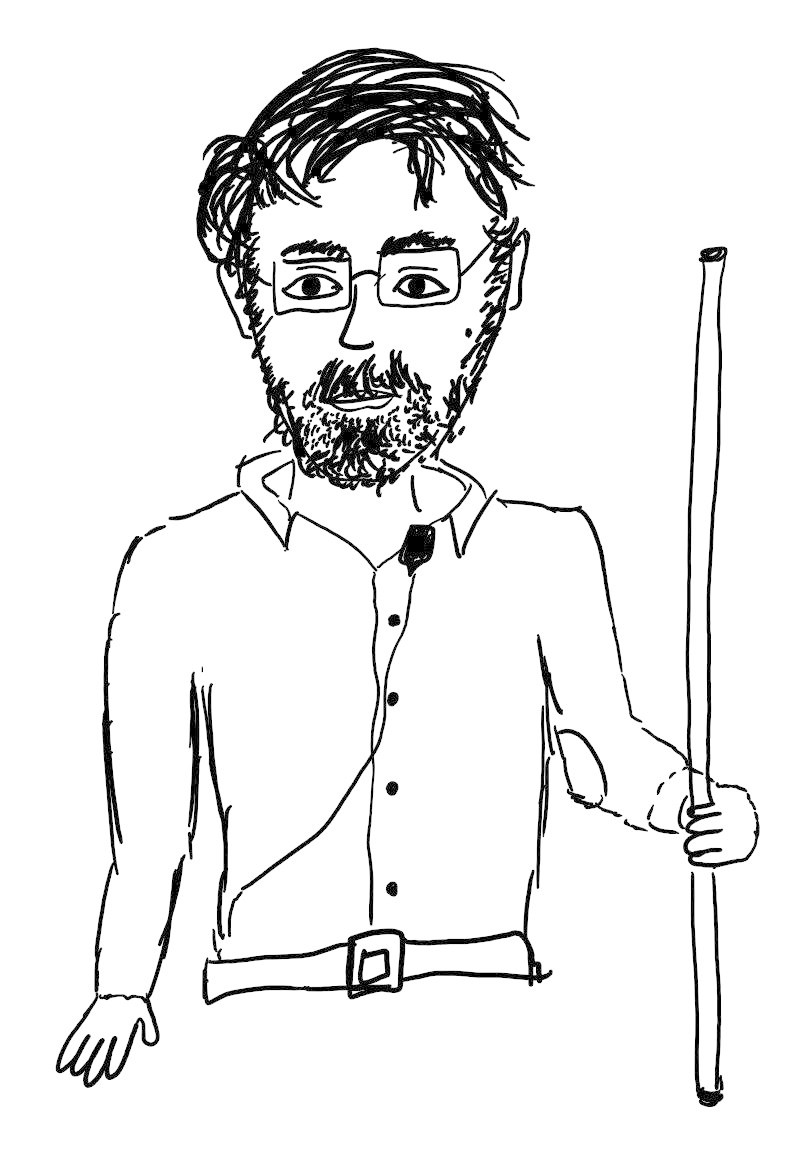
\includegraphics[width=0.1\linewidth]{../you_light}}

\date{20/05/2019}
\institute[PoliMi]{\vspace{0.5cm}Politecnico di Milano}
\logo{
\includegraphics[width=10mm]{../logopolimi_light}}

\setbeamercovered{invisible}

\makeindex

\begin{document}
\begin{frame}
	\maketitle
\end{frame}

\begin{frame}{Recap - Unbalanced systems}
\begin{enumerate}
	\item Calculate $D = \sum_{k=1}^K D_k$ and $D_{max} = \max_k{D_k}$
	\item Calculate the intersection point $N^* = \frac{D+Z}{D_{max}}$
	\item Compute bounds for throughput and response time
\end{enumerate}

\bgroup
\def\arraystretch{1.2}
\begin{tabular}{|c|c|}
	\hline
	batch & $\frac{1}{D} \leq X(N) \leq \min{(\frac{N}{D}, \frac{1}{D_{max}})}$ \\
	terminal & $\frac{N}{ND+Z} \leq X(N) \leq \min{(\frac{N}{D+Z}, \frac{1}{D_{max}})}$ \\
	transaction	&	$X(\lambda) \leq \frac{1}{D_{max}}$ \\
	\hline
\end{tabular}

\begin{tabular}{|c|c|}
	\hline
	batch & $\max{(D, ND_{max})} \leq R(N) \leq ND$ \\
	terminal & $\max{(D, ND_{max} - Z)} \leq R(N) \leq ND$ \\
	transaction	&	$D \leq R(\lambda)$ \\
	\hline
\end{tabular}
\egroup

Tighter bounds hold for balanced systems.
\end{frame}

\begin{frame}{Exercise 1}
An intranet is composed of 5 web servers used in parallel, 3 application servers used in parallel, and 1 storage server. The other components on the intranet (e.g., switches, gateways, load balancers, firewalls,
network) are not considered since their utilization is very low.
The servers connected in parallel are used in a
balanced way. The complete execution of a transaction requires (service demands) 750 ms to the web
server, 600 ms to the application server and 300 ms to the storage server.

Compute the maximum throughput of the intranet.

Derive bounds on throughput and response time assuming $Z=0$
\end{frame}

\begin{frame}{Solution}
$D_{ws} = \frac{750ms}{5} = 150ms$
$D_{as} = \frac{600ms}{3} = 200ms$
$D_{ss} = 300ms$

$X_{max} = \frac{1}{D_{max}} = \frac{1}{0.3 sec} = 3.3 sec$

$\color{red}\frac{1}{D} \color{black}\leq X(N) \leq \max(\color{green}\frac{N}{D}, \color{blue} \frac{1}{D_{max}})$
$\max(\color{green}D, \color{red} N D_{max} \color{black}) \leq R(N) \leq \color{blue} ND$

$D = \sum D_i = 650ms$ $D_{max} = 300ms$ $N^*=\frac{D+Z}{D_{max}} = 2.16$ $\frac{1}{D} = 1.54$ $\frac{1}{D_{max}} = 3.3$

\begin{tikzpicture}[scale=0.5]
\draw[->] (0,0) -- (5,0) node[right] {$N$};
\draw[->] (0,0) -- (0,5) node[above] {$X$};

\draw[blue] (2.16, 3.3) -- (5, 3.3);
\draw[green] (1, 1.54) -- (2.16, 3.3);
\draw[red] (1, 1.54) -- (5, 1.54);

\draw (1,-0.2) -- (1, 0.2);
\node[anchor=north] at (1,0) {1};
\draw (2.16,-0.2) -- (2.16, 0.2);
\node[anchor=north] at (2.16, 0) {$N^*$};

\draw (-0.2, 1.54) -- (0.2, 1.54);
\node[anchor=east] at (0,1.54) {$\frac{1}{D}$};
\draw (-0.2, 3.3) -- (0.2, 3.3);
\node[anchor=east] at (0, 3.3) {$\frac{1}{D_{max}}$};
\end{tikzpicture}
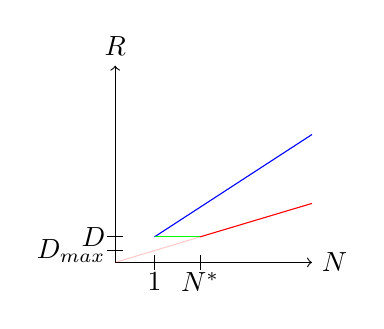
\begin{tikzpicture}[scale=0.5]
\draw[->] (0,0) -- (5,0) node[right] {$N$};
\draw[->] (0,0) -- (0,5) node[above] {$R$};

\draw[blue] (1, 0.65) -- (5, 5*0.65);
\draw[green] (1, 0.65) -- (2.16, 0.65);
\draw[red] (2.16, 0.65) -- (5, 5*0.3);
\draw[red, opacity=0.2] (0,0) -- (2.16, 0.65);

\draw (1,-0.2) -- (1, 0.2);
\node[anchor=north] at (1,0) {1};
\draw (2.16,-0.2) -- (2.16, 0.2);
\node[anchor=north] at (2.16, 0) {$N^*$};

\draw (-0.2, 0.3) -- (0.2, 0.3);
\node[anchor=east] at (0,0.3) {$D_{max}$};
\draw (-0.2, 0.65) -- (0.2, 0.65);
\node[anchor=east] at (0, 0.65) {$D$};
\end{tikzpicture}
\end{frame}

\begin{frame}[allowframebreaks]{Exercise 2}
Let’s consider an IT infrastructure consisting of a Web Server (WS), an Application Server (AS) and a Storage Server (SS).

After 1 hour measurement, during which N = 50 users were working continuously, the following
data have been collected:
\begin{itemize}
\item $C$ total number of jobs executed by the system: 5400 j
\item $C_{WS}$ Number of WS completed operations: 54000 op
\item $C_{AS}$ Number of AS completed operations: 32400 op
\item $C_{SS}$ Number of SS completed operations: 10800 op
\item $B_{WS}$ WS total activity time: 1800 sec
\item $B_{AS}$ AS total activity time: 720 sec
\item $B_{SS}$ SS total activity time: 900 sec
\item $Z$ Mean think time 5 sec
\end{itemize}

Using Operational Analysis equations:
\begin{enumerate}
\item Compute the visits $V_i$ to the three servers during a complete job execution, their global service requests $D_i$ and determine the bottleneck resource of the IT infrastructure
\item Compute response time when $N = 50$ users are connected, as well as the maximum throughput when the number of users tends to infinity (asymptotic value)
\item Let’s substitute the bottleneck resource determined at point 1 with another, two times (2x) more powerful. Does the bottleneck migrate to another resource? If so, which one? Compute the new value of the asymptotic throughput.
\end{enumerate}
\end{frame}

\begin{frame}[allowframebreaks]{Solution}
Point 1:\\
$V_i = \frac{C_i}{C} \rightarrow V_{ws} = 10 \quad V_{as} = 6 \quad V_{ss} = 2$

$D_i = \frac{U_i}{X} \qquad X= \frac{C}{T} = 1.5$
$U_i = \frac{B_i}{T} \rightarrow U_{ws} = 0.5 \quad U_{as}=0.2 \quad U_{ss} = 0.25$
$D_{ws} = 0.33 \quad D_{as} = 0.13 \quad D_{ss} = 0.16$

$D_{max} = D_{ws} = 0.33$

Point 2:\\
$R(50) = \frac{N}{X}-Z = 28.3 sec$ \ \ \
$X_{max} = \frac{1}{D_{max}} = 3 \frac{job}{sec}$

Point 3:\\
$D'_{ws} = 0.16 sec \rightarrow $ new bottlenecks are ws and ss. \ \ \
$X'_{max} = 6 \frac{job}{sec}$

\break

\begin{tabular}{|c|c|c|c|c|c|c|}
	\hline
	System	&	$D$	&	$D_{max}$	&	$N^*$	&	$\frac{1}{D}$	&	$\frac{1}{D+Z}$	&	$\frac{1}{D_{max}}$	\\
	\hline
	\color{blue}Original &	0.633	&	0.333	&	16.9	&	1.58	&	0.17	&	3	\\
	\color{red}Modified &	0.466	&	0.166	&	32.9	&	2.14	&	0.18	&	6	\\
	\hline
\end{tabular}

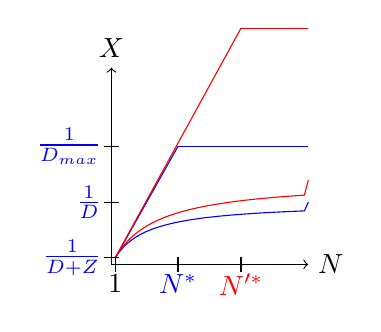
\begin{tikzpicture}[scale=0.5]
\draw[->] (0,0) -- (5,0) node[right] {$N$};
\draw[->] (0,0) -- (0,5) node[above] {$X$};

\draw[blue] (1.69, 3) -- (5, 3);
\draw[blue] (0.1, 0.17) -- (1.69, 3);
\draw[blue, smooth] (0.100000, 0.177525)--(0.200000, 0.319183)--(0.300000, 0.434846)--(0.400000, 0.531067)--(0.500000, 0.612370)--(0.600000, 0.681973)--(0.700000, 0.742233)--(0.800000, 0.794913)--(0.900000, 0.841357)--(1.000000, 0.882613)--(1.100000, 0.919502)--(1.200000, 0.952683)--(1.300000, 0.982690)--(1.400000, 1.009955)--(1.500000, 1.034840)--(1.600000, 1.057641)--(1.700000, 1.078612)--(1.800000, 1.097963)--(1.900000, 1.115875)--(2.000000, 1.132503)--(2.100000, 1.147980)--(2.200000, 1.162422)--(2.300000, 1.175929)--(2.400000, 1.188590)--(2.500000, 1.200480)--(2.600000, 1.211669)--(2.700000, 1.222217)--(2.800000, 1.232177)--(2.900000, 1.241598)--(3.000000, 1.250521)--(3.100000, 1.258986)--(3.200000, 1.267026)--(3.300000, 1.274673)--(3.400000, 1.281955)--(3.500000, 1.288897)--(3.600000, 1.295523)--(3.700000, 1.301854)--(3.800000, 1.307909)--(3.900000, 1.313706)--(4.000000, 1.319261)--(4.100000, 1.324589)--(4.200000, 1.329703)--(4.300000, 1.334616)--(4.400000, 1.339340)--(4.500000, 1.343885)--(4.600000, 1.348262)--(4.700000, 1.352479)--(4.800000, 1.356545)--(4.900000, 1.360469)--(5,1.58);

\draw[red] (3.29, 6) -- (5, 6);
\draw[red] (0.1, 0.18) -- (3.29, 6);
\draw[red, smooth] (0.100000, 0.182949)--(0.200000, 0.337154)--(0.300000, 0.468897)--(0.400000, 0.582751)--(0.500000, 0.682128)--(0.600000, 0.769625)--(0.700000, 0.847252)--(0.800000, 0.916590)--(0.900000, 0.978899)--(1.000000, 1.035197)--(1.100000, 1.086312)--(1.200000, 1.132931)--(1.300000, 1.175619)--(1.400000, 1.214856)--(1.500000, 1.251043)--(1.600000, 1.284522)--(1.700000, 1.315586)--(1.800000, 1.344488)--(1.900000, 1.371445)--(2.000000, 1.396648)--(2.100000, 1.420262)--(2.200000, 1.442434)--(2.300000, 1.463290)--(2.400000, 1.482946)--(2.500000, 1.501502)--(2.600000, 1.519047)--(2.700000, 1.535661)--(2.800000, 1.551418)--(2.900000, 1.566382)--(3.000000, 1.580611)--(3.100000, 1.594158)--(3.200000, 1.607071)--(3.300000, 1.619393)--(3.400000, 1.631165)--(3.500000, 1.642421)--(3.600000, 1.653196)--(3.700000, 1.663519)--(3.800000, 1.673419)--(3.900000, 1.682921)--(4.000000, 1.692047)--(4.100000, 1.700821)--(4.200000, 1.709263)--(4.300000, 1.717390)--(4.400000, 1.725220)--(4.500000, 1.732769)--(4.600000, 1.740051)--(4.700000, 1.747082)--(4.800000, 1.753873)--(4.900000, 1.760437)--(5, 2.14);

\draw (0.1,-0.2) -- (0.1, 0.2);
\node[anchor=north] at (0.1,0) {1};
\draw (1.69,-0.2) -- (1.69, 0.2);
\node[anchor=north, color=blue] at (1.69, 0) {$N^*$};
\draw (3.29,-0.2) -- (3.29, 0.2);
\node[anchor=north, color=red] at (3.29, 0) {$N'^*$};

\draw (-0.2, 0.17) -- (0.2, 0.17);
\node[anchor=east, color=blue] at (0,0.17) {$\frac{1}{D+Z}$};
\draw (-0.2, 1.58) -- (0.2, 1.58);
\node[anchor=east, color=blue] at (0,1.58) {$\frac{1}{D}$};
\draw (-0.2, 3) -- (0.2, 3);
\node[anchor=east, color=blue] at (0, 3) {$\frac{1}{D_{max}}$};
\end{tikzpicture}
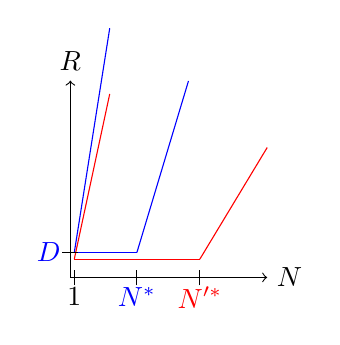
\begin{tikzpicture}[scale=0.5]
\draw[->] (0,0) -- (5,0) node[right] {$N$};
\draw[->] (0,0) -- (0,5) node[above] {$R$};

\draw[blue] (0.1, 0.633) -- (1, 10*0.633);
\draw[blue] (0.1, 0.633) -- (1.69, 0.633);
\draw[blue] (1.69, 0.633) -- (3, 30*0.333-5);

\draw[red] (0.1, 0.466) -- (1, 10*0.466);
\draw[red] (0.1, 0.466) -- (3.29, 0.466);
\draw[red] (3.29, 0.466) -- (5, 50*0.166-5);

\draw (0.1,-0.2) -- (0.1, 0.2);
\node[anchor=north] at (0.1,0) {1};
\draw (1.69,-0.2) -- (1.69, 0.2);
\node[anchor=north, color=blue] at (1.69, 0) {$N^*$};
\draw (3.29,-0.2) -- (3.29, 0.2);
\node[anchor=north, color=red] at (3.29, 0) {$N'^*$};

\draw (-0.2, 0.633) -- (0.2, 0.633);
\node[anchor=east, color=blue] at (0,0.633) {$D$};
\end{tikzpicture}
\end{frame}

\begin{frame}{Exercise 3}
Let’s consider an intranet that can be accessed by a large number of users. The execution of a single
request pass through an application server (AS), which has a service time $S = 300 ms$, then through a database server (DS), which has a service time $S = 250 ms$, and then back through the application server. A request must pass through the system firewall before entering the intranet and before exiting from it. The
firewall service time per visit is $S = 10 ms$.
\begin{enumerate}
	\item Compute the maximum throughput of the system.
	\item Is it possible to have a Response Time $R < 9s$? At which conditions?
\end{enumerate}
\end{frame}

\begin{frame}{Solutions}
$D_i = S_i V_i \rightarrow D_{as} = 600ms \quad D_{ds}=250ms \quad D_{fw} = 20ms$

Assuming a closed system with $Z=0$ we need: $\max(D, ND_{max}) \leq R(N) \rightarrow ND_{max} \leq 9 \rightarrow N \leq 15$
\end{frame}

\begin{frame}{Exercise 4}
A session of a graphical multi-user workstation, using a disk with an average service time $S_{disk} = 25 ms$, yields the following measurements:
\begin{itemize}
\item average think-time $z = 10 s$
\item average CPU service demand, $D_{cpu} = 4 s$
\item average disk service demand, $D_{disk} = 5 s$
\item fraction of the busy time in which the CPU performs floating point operations 75\%
\end{itemize}

Evaluate, using asymptotic bounds, which of the following modifications is more advantageous:
\begin{enumerate}
	\item adding a FPU, which is 10 times as fast as the CPU, to offload floating point operations
	\item replacing the disk with a new one with $S'_{disk} = 15 ms$
\end{enumerate}
\end{frame}

\begin{frame}[allowframebreaks]{Solution}
Adding a fpu:\\
$D'_{cpu} = \frac{D_{cpu}}{4} = 1 sec \qquad D_{fpu} = \frac{\frac{3 D_{cpu}}{4}}{10} = 0.3 sec$

Replacing the disk:\\
$V_{disk} = \frac{D_{disk}}{S_{disk}} = 200 \qquad D'_{disk} = V_{disk} S'_{disk} = 3s$

\break

\begin{tabular}{|c|c|c|c|c|c|c|}
	\hline
	System	&	$D$	&	$D_{max}$	&	$N^*$	&	$\frac{1}{D}$	&	$\frac{1}{D+Z}$	&	$\frac{1}{D_{max}}$	\\
	\hline
	\color{red}Original&9	&	5	&	3.8		&	0.111	&	0.053	&	0.2	\\
	\color{green}FPU &	6.3	&	5	&	3.26	&	0.159	&	0.061	&	0.2	\\
	\color{blue}Disk &	7	&	4	&	4.25	&	0.143	&	0.059	&	0.25 \\
	\hline
\end{tabular}

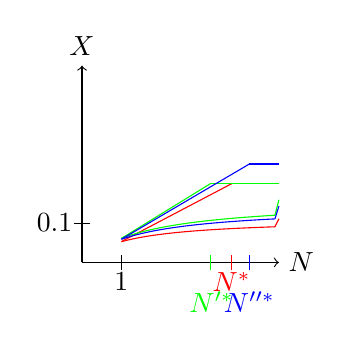
\begin{tikzpicture}[scale=0.5]
\draw[->] (0,0) -- (5,0) node[right] {$N$};
\draw[->] (0,0) -- (0,5) node[above] {$X$};

\draw[red] (3.8, 2) -- (5, 2);
\draw[red] (1, 0.53) -- (3.8, 2);
\draw[red, smooth] (1.000000, 0.526316)--(1.100000, 0.552764)--(1.200000, 0.576923)--(1.300000, 0.599078)--(1.400000, 0.619469)--(1.500000, 0.638298)--(1.600000, 0.655738)--(1.700000, 0.671937)--(1.800000, 0.687023)--(1.900000, 0.701107)--(2.000000, 0.714286)--(2.100000, 0.726644)--(2.200000, 0.738255)--(2.300000, 0.749186)--(2.400000, 0.759494)--(2.500000, 0.769231)--(2.600000, 0.778443)--(2.700000, 0.787172)--(2.800000, 0.795455)--(2.900000, 0.803324)--(3.000000, 0.810811)--(3.100000, 0.817942)--(3.200000, 0.824742)--(3.300000, 0.831234)--(3.400000, 0.837438)--(3.500000, 0.843373)--(3.600000, 0.849057)--(3.700000, 0.854503)--(3.800000, 0.859729)--(3.900000, 0.864745)--(4.000000, 0.869565)--(4.100000, 0.874200)--(4.200000, 0.878661)--(4.300000, 0.882957)--(4.400000, 0.887097)--(4.500000, 0.891089)--(4.600000, 0.894942)--(4.700000, 0.898662)--(4.800000, 0.902256)--(4.900000, 0.905730)--(5.0, 1.11);

\draw[green] (3.26, 2) -- (5, 2);
\draw[green] (1, 0.61) -- (3.26, 2);
\draw[green, smooth] (1.000000, 0.613497)--(1.100000, 0.649734)--(1.200000, 0.683371)--(1.300000, 0.714678)--(1.400000, 0.743889)--(1.500000, 0.771208)--(1.600000, 0.796813)--(1.700000, 0.820859)--(1.800000, 0.843486)--(1.900000, 0.864816)--(2.000000, 0.884956)--(2.100000, 0.904003)--(2.200000, 0.922045)--(2.300000, 0.939159)--(2.400000, 0.955414)--(2.500000, 0.970874)--(2.600000, 0.985595)--(2.700000, 0.999630)--(2.800000, 1.013025)--(2.900000, 1.025822)--(3.000000, 1.038062)--(3.100000, 1.049780)--(3.200000, 1.061008)--(3.300000, 1.071777)--(3.400000, 1.082113)--(3.500000, 1.092044)--(3.600000, 1.101591)--(3.700000, 1.110778)--(3.800000, 1.119623)--(3.900000, 1.128146)--(4.000000, 1.136364)--(4.100000, 1.144292)--(4.200000, 1.151947)--(4.300000, 1.159342)--(4.400000, 1.166490)--(4.500000, 1.173403)--(4.600000, 1.180092)--(4.700000, 1.186569)--(4.800000, 1.192843)--(4.900000, 1.198923)--(5.0, 1.59);

\draw[blue] (4.25, 2.5) -- (5, 2.5);
\draw[blue] (1, 0.59) -- (4.25, 2.5);
\draw[blue, smooth] (1.000000, 0.588235)--(1.100000, 0.621469)--(1.200000, 0.652174)--(1.300000, 0.680628)--(1.400000, 0.707071)--(1.500000, 0.731707)--(1.600000, 0.754717)--(1.700000, 0.776256)--(1.800000, 0.796460)--(1.900000, 0.815451)--(2.000000, 0.833333)--(2.100000, 0.850202)--(2.200000, 0.866142)--(2.300000, 0.881226)--(2.400000, 0.895522)--(2.500000, 0.909091)--(2.600000, 0.921986)--(2.700000, 0.934256)--(2.800000, 0.945946)--(2.900000, 0.957096)--(3.000000, 0.967742)--(3.100000, 0.977918)--(3.200000, 0.987654)--(3.300000, 0.996979)--(3.400000, 1.005917)--(3.500000, 1.014493)--(3.600000, 1.022727)--(3.700000, 1.030641)--(3.800000, 1.038251)--(3.900000, 1.045576)--(4.000000, 1.052632)--(4.100000, 1.059432)--(4.200000, 1.065990)--(4.300000, 1.072319)--(4.400000, 1.078431)--(4.500000, 1.084337)--(4.600000, 1.090047)--(4.700000, 1.095571)--(4.800000, 1.100917)--(4.900000, 1.106095)--(5.0, 1.43);

\draw (1,-0.2) -- (1, 0.2);
\node[anchor=north] at (1,0) {1};
\draw[color=red] (3.8,-0.2) -- (3.8, 0.2);
\node[anchor=north, color=red] at (3.8, 0) {$N^*$};
\draw[color=green] (3.26,-0.2) -- (3.26, 0.2);
\node[anchor=north, color=green] at (3.29, -0.5) {$N'^*$};
\draw[color=blue] (4.25,-0.2) -- (4.25, 0.2);
\node[anchor=north, color=blue] at (4.25, -0.5) {$N''^*$};

\draw (-0.2, 1) -- (0.2, 1);
\node[anchor=east] at (0,1) {0.1};
\end{tikzpicture}
\hspace{1cm}
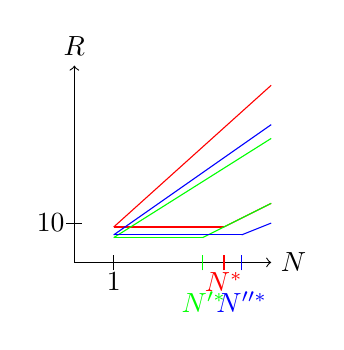
\begin{tikzpicture}[scale=0.5]
\draw[->] (0,0) -- (5,0) node[right] {$N$};
\draw[->] (0,0) -- (0,5) node[above] {$R$};

\draw[red] (1, 0.9) -- (5, 5*9/10);
\draw[red] (1, 0.9) -- (3.8, 0.9);
\draw[red] (3.8, 0.9) -- (5, 0.5*5-1);

\draw[green] (1, 0.63) -- (5, 5*6.3/10);
\draw[green] (1, 0.63) -- (3.26, 0.63);
\draw[green] (3.26, 0.63) -- (5, 0.5*5-1);

\draw[blue] (1, 0.7) -- (5, 5*7/10);
\draw[blue] (1, 0.7) -- (4.25, 0.7);
\draw[blue] (4.25, 0.7) -- (5, 0.5*4-1);

\draw (1,-0.2) -- (1, 0.2);
\node[anchor=north] at (1,0) {1};
\draw[color=red] (3.8,-0.2) -- (3.8, 0.2);
\node[anchor=north, color=red] at (3.8, 0) {$N^*$};
\draw[color=green] (3.26,-0.2) -- (3.26, 0.2);
\node[anchor=north, color=green] at (3.29, -0.5) {$N'^*$};
\draw[color=blue] (4.25,-0.2) -- (4.25, 0.2);
\node[anchor=north, color=blue] at (4.25, -0.5) {$N''^*$};

\draw (-0.2, 1) -- (0.2, 1);
\node[anchor=east] at (0,1) {10};
\end{tikzpicture}
\end{frame}


\begin{frame}[allowframebreaks]{Exercise 5}
Consider a web application deployment structured as follows:
\begin{itemize}
\item one web server (WS) that renders dynamic pages,
\item one application server (AS) that constructs such dynamic pages,
\item  one database server (DB) that holds the data needed by the application server.
\end{itemize}
The web server is the most demanded center, it has indeed $D_{WS} = 5ms$.
The application server and the database server have a service demand of, respectively,
$D_{AS} = 4ms$ and $D_{DB} = 3ms$.

The we application is tested in a closed deployment with a terminal workload of 20 customers
with a think time of 7 milliseconds.

\begin{enumerate}
\item  What is the primary bottleneck center?
\item  What is the secondary bottleneck center?
\item  What is the minimum response time that can be achieved?
\item  What is the effect of replacing the application server with a new one that is twice as fast?
\item What is the modification, if any, that would allow the application server to run at its maximum speed?
\end{enumerate}
\end{frame}

\begin{frame}[allowframebreaks]{Solutions}
$D_{max} = D_{ws} \rightarrow X_{max} = \frac{1}{D_{max}} = 200 r/s$

$D'_{max} = D_{as} \rightarrow X'_{max} = \frac{1}{D'_{max}} = 250 r/s$

$R_{min} = D = 12ms \quad (R \geq \max(D, N D_{max} - Z))$

\break
$D'_{as} = 2ms$ does not modify $X_{max}$ as the AS is not the bottleneck. However, $D$ changes and therefore there is a (small) difference in the graphs:

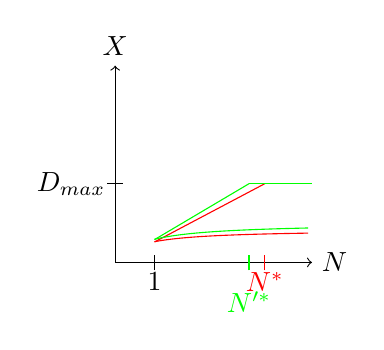
\begin{tikzpicture}[scale=0.5]
\draw[->] (0,0) -- (5,0) node[right] {$N$};
\draw[->] (0,0) -- (0,5) node[above] {$X$};

\draw[red] (3.8, 2) -- (5, 2);
\draw[red] (1, 0.52) -- (3.8, 2);
\draw[red, smooth] (1.000000, 0.526316)--(1.100000, 0.544554)--(1.200000, 0.560748)--(1.300000, 0.575221)--(1.400000, 0.588235)--(1.500000, 0.600000)--(1.600000, 0.610687)--(1.700000, 0.620438)--(1.800000, 0.629371)--(1.900000, 0.637584)--(2.000000, 0.645161)--(2.100000, 0.652174)--(2.200000, 0.658683)--(2.300000, 0.664740)--(2.400000, 0.670391)--(2.500000, 0.675676)--(2.600000, 0.680628)--(2.700000, 0.685279)--(2.800000, 0.689655)--(2.900000, 0.693780)--(3.000000, 0.697674)--(3.100000, 0.701357)--(3.200000, 0.704846)--(3.300000, 0.708155)--(3.400000, 0.711297)--(3.500000, 0.714286)--(3.600000, 0.717131)--(3.700000, 0.719844)--(3.800000, 0.722433)--(3.900000, 0.724907)--(4.000000, 0.727273)--(4.100000, 0.729537)--(4.200000, 0.731707)--(4.300000, 0.733788)--(4.400000, 0.735786)--(4.500000, 0.737705)--(4.600000, 0.739550)--(4.700000, 0.741325)--(4.800000, 0.743034)--(4.900000, 0.744681);

\draw[green] (3.4, 2) -- (5, 2);
\draw[green] (1, 0.58) -- (3.4, 2);
\draw[green, smooth] (1.000000, 0.588235)--(1.100000, 0.611111)--(1.200000, 0.631579)--(1.300000, 0.650000)--(1.400000, 0.666667)--(1.500000, 0.681818)--(1.600000, 0.695652)--(1.700000, 0.708333)--(1.800000, 0.720000)--(1.900000, 0.730769)--(2.000000, 0.740741)--(2.100000, 0.750000)--(2.200000, 0.758621)--(2.300000, 0.766667)--(2.400000, 0.774194)--(2.500000, 0.781250)--(2.600000, 0.787879)--(2.700000, 0.794118)--(2.800000, 0.800000)--(2.900000, 0.805556)--(3.000000, 0.810811)--(3.100000, 0.815789)--(3.200000, 0.820513)--(3.300000, 0.825000)--(3.400000, 0.829268)--(3.500000, 0.833333)--(3.600000, 0.837209)--(3.700000, 0.840909)--(3.800000, 0.844444)--(3.900000, 0.847826)--(4.000000, 0.851064)--(4.100000, 0.854167)--(4.200000, 0.857143)--(4.300000, 0.860000)--(4.400000, 0.862745)--(4.500000, 0.865385)--(4.600000, 0.867925)--(4.700000, 0.870370)--(4.800000, 0.872727)--(4.900000, 0.875000);

\draw (1,-0.2) -- (1, 0.2);
\node[anchor=north] at (1,0) {1};

\draw[color=red] (3.8,-0.2) -- (3.8, 0.2);
\node[anchor=north, color=red] at (3.8, 0) {$N^*$};
\draw[color=green] (3.4,-0.2) -- (3.4, 0.2);
\node[anchor=north, color=green] at (3.4, -0.5) {$N'^*$};

\draw (-0.2, 2) -- (0.2, 2);
\node[anchor=east] at (0,2) {$D_{max}$};
\end{tikzpicture}
\hspace{1cm}
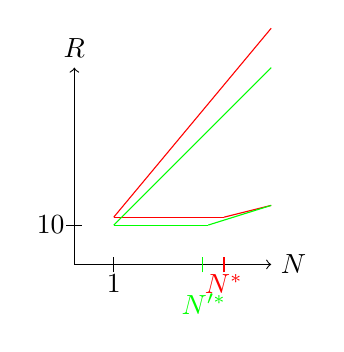
\begin{tikzpicture}[scale=0.5]
\draw[->] (0,0) -- (5,0) node[right] {$N$};
\draw[->] (0,0) -- (0,5) node[above] {$R$};

\draw[red] (1, 1.2) -- (5, 5*12/10);
\draw[red] (1, 1.2) -- (3.8, 1.2);
\draw[red] (3.8, 1.2) -- (5, 0.5*5-1);

\draw[green] (1, 1) -- (5, 5*10/10);
\draw[green] (1, 1) -- (3.4, 1);
\draw[green] (3.4, 1) -- (5, 0.5*5-1);


\draw (1,-0.2) -- (1, 0.2);
\node[anchor=north] at (1,0) {1};
\draw[color=red] (3.8,-0.2) -- (3.8, 0.2);
\node[anchor=north, color=red] at (3.8, 0) {$N^*$};
\draw[color=green] (3.26,-0.2) -- (3.26, 0.2);
\node[anchor=north, color=green] at (3.29, -0.5) {$N'^*$};

\draw (-0.2, 1) -- (0.2, 1);
\node[anchor=east] at (0,1) {10};
\end{tikzpicture}

\end{frame}

\begin{frame}[allowframebreaks]{Exercise 6}
A website is deployed onto a machine that runs one instance of the Nginx3 web server and two parallel instances of the PostgreSQL4 database server (each on a separate disk).

In our closed, terminal workload environment, we simulated the activity of $N$ clients
with 15 seconds of think time and we measured the busy time and the number of jobs
completed at each center (except for the web server) for a time interval of 900 seconds.
During this time interval the system rendered 200 HTTP responses back to the clients.

The measurements were as follows:
\begin{itemize}
\item  the web server has a busy time of 400 seconds,
\item  the first database server has a busy time of 100 seconds, and completed 2000
operations,
\item the second database server has a busy time of 600 seconds, and completed 20000
operations.
\end{itemize}

\begin{enumerate}
\item
Can you spot the bottleneck?
\item
How many visits, to each database server, are required per HTTP request?
\item
How much service time does a visit take on each database server?
\item
What is the effect of replacing the Nginx web server with the Cherokee5 web server,
which is twice as fast?
\item
The database administrator claims that the load between the two database servers
is perfectly balanced. Is he correct? Why?
\item
If you are given enough money to buy a new disk to run an additional database
server, how would you modify the system?
\item
What would be a non-obtrusive modification (i.e., involving no costs at all) to
alleviate the bottleneck?
\end{enumerate}
\end{frame}

\begin{frame}{Solutions}
\begin{enumerate}
\item $D_i = \frac{B_i}{C} \rightarrow D_{ws} = 2sec \quad D_{db1} = 0.5 sec \quad D_{db2} = 3 sec$
$D_{max} = D_{db2} = 3 sec \rightarrow X_{max} = 0.3j/sec$

\item $V_i = \frac{C_i}{C} \rightarrow V_{db1} = 10 \quad V_{db2} = 100$

\item $S_i = \frac{D_i}{V_i} \rightarrow S_{db1} = 50ms \quad S_{db2} = 30ms$

\item $D'_{ws} = 1 sec$ but $D_{max}$ does not change.

\item The second database has 6 times the demand of the first one, so they are by no means balanced.

\item We could split the load of the second database

\item We want $D'_{db1} = D'_{db2} = d$ and $V_{db1} + V_{db2} = V'_{db1} + v'_{db2} = 110$
$\rightarrow V'_{db1} \frac{S_{db1}}{S_{db1}} + V'_{db2} \frac{S_{db2}}{S_{db2}} = 110$
$\rightarrow \frac{D'_{db1}}{S_{db1}} + \frac{D'_{db2}}{S_{db2}} = 110$
$\rightarrow d (\frac{1}{S_{db1}} + \frac{1}{S_{db2}})  = 110$
$\rightarrow d = 2.07 sec$ and $X_{max} = 0.48j/sec$
\end{enumerate}
\end{frame}
\end{document}
